\documentclass[12pt]{article}

\usepackage[utf8]{inputenc}
\usepackage[brazil]{babel}
\usepackage[a4paper,left=3cm, right=2cm,top=2.5cm, bottom=2.5cm]{geometry}
\usepackage{amsmath}
\usepackage{graphicx}
\usepackage{float}
\usepackage{multirow}
\usepackage{authblk}
\usepackage{fancyhdr}
\usepackage{xcolor}
\usepackage{cite}


\title{\textbf{ENG1456 - Lógica Fuzzy - Trabalho 2}}
\author{\textbf{Aluno: Matheus Carneiro Nogueira - 1810764}}
\affil{}
\author{\textbf{Professora: Ricardo Tanscheit}}
\affil{}
\pagestyle{fancy}
\fancyhf{}
\lhead{{\small \textcolor{gray}{PUC-Rio ENG1456}}}
\renewcommand{\headrulewidth}{0pt}
\date{}
\renewcommand{\footrulewidth}{0pt}
\fancyfoot[C]{\thepage}

\begin{document}
	\maketitle
	\tableofcontents
	

\begin{abstract}
	Este documento consiste no relatório do trabalho 2 do módulo de Lógica Fuzzy da disciplina ENG1456 da PUC-Rio. O trabalho é dividido em duas partes. Primeiramente, o objetivo é alterar o banco de regras em duas situações distintas com o intuito de fazer o container ser parar no local correto. A segunda parte consiste em calcular manualmente as saídas de cada base de regras e a resposta final do sistema de inferência para as variáveis definidas no problema imobiliário. Será utilizado o software Fuzzytech para a realização deste trabalho.
\end{abstract}

\section{Parte 1 - Controle do Guindaste}

\subsection{QR 1 - Exibindo estado inicial}

Antes de alterar o banco de regras do sistema de controle fuzzy para o controle do guindaste, as figuras abaixo exibem o estado inicial dessas regras. Além disso, também é exibida uma figura que mostra a posição final do container na situação 1.
\begin{figure}[H]
	\centering
	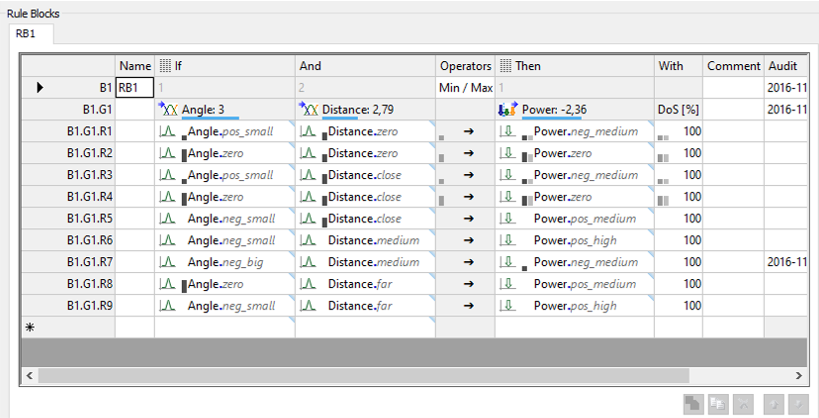
\includegraphics[width=0.9\linewidth]{Imagens/QR1/regrasOriginais}
	\caption{Regras originais}
	\label{fig:regrasoriginais}
\end{figure}
\begin{figure}[H]
	\centering
	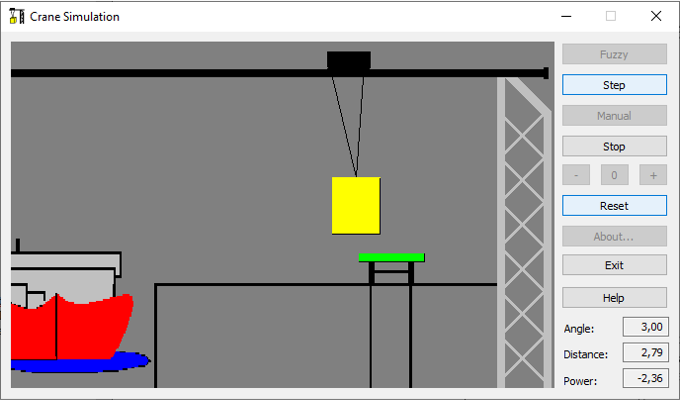
\includegraphics[width=0.9\linewidth]{Imagens/QR1/posicaoFinalOriginal}
	\caption{Posição Final original do container}
	\label{fig:posicaoFinalOriginal}
\end{figure}

A partir da figura \ref{fig:posicaoFinalOriginal} pode-se perceber que o guindaste parou antes da posição correta. Vale a pena, antes de mudar as regras arbitrariamente,  analisar as regras originais para tentar encontrar alguma regra mal definida.

Primeiramente, nota-se que existem duas regras cuja consequência é \textit{Power.zero}. São elas:
\begin{align*}
	Angle.zero\&Distance.zero\to Power.zero\\
	Angle.zero\&Distance.close\to Power.zero
\end{align*}

A primeira regra faz sentido, uma vez que os dois antecedentes indicam que o guindaste chegou na posição correta, o que implica que ele deve ser desligado. A segunda, por outro lado, é estranha. Ao se aproximar do local destino, isto é, à medida que a distância fica próxima, é natural que queiramos diminuir a potência do guindaste, mas não zerá-la completamente. Essa será a primeira regra a ser alterada.

\subsection{QR 1 - Alteração de Regras}

Como comentado, a primeira alteração a ser feita é alterar a regra $(1)$ abaixo. Como o guindaste parou um pouco antes do local adequado, alteremos essa regra para $(2)$, pois queremos que o guindaste ainda ande um pouco para a direita.

\begin{align}
	Angle.zero\&Distance.close&\to Power.zero\\
	Angle.zero\&Distance.close&\to Power.pos\_medium
\end{align}

O resultado dessa alteração é exibido na figura abaixo.
\begin{figure}[H]
	\centering
	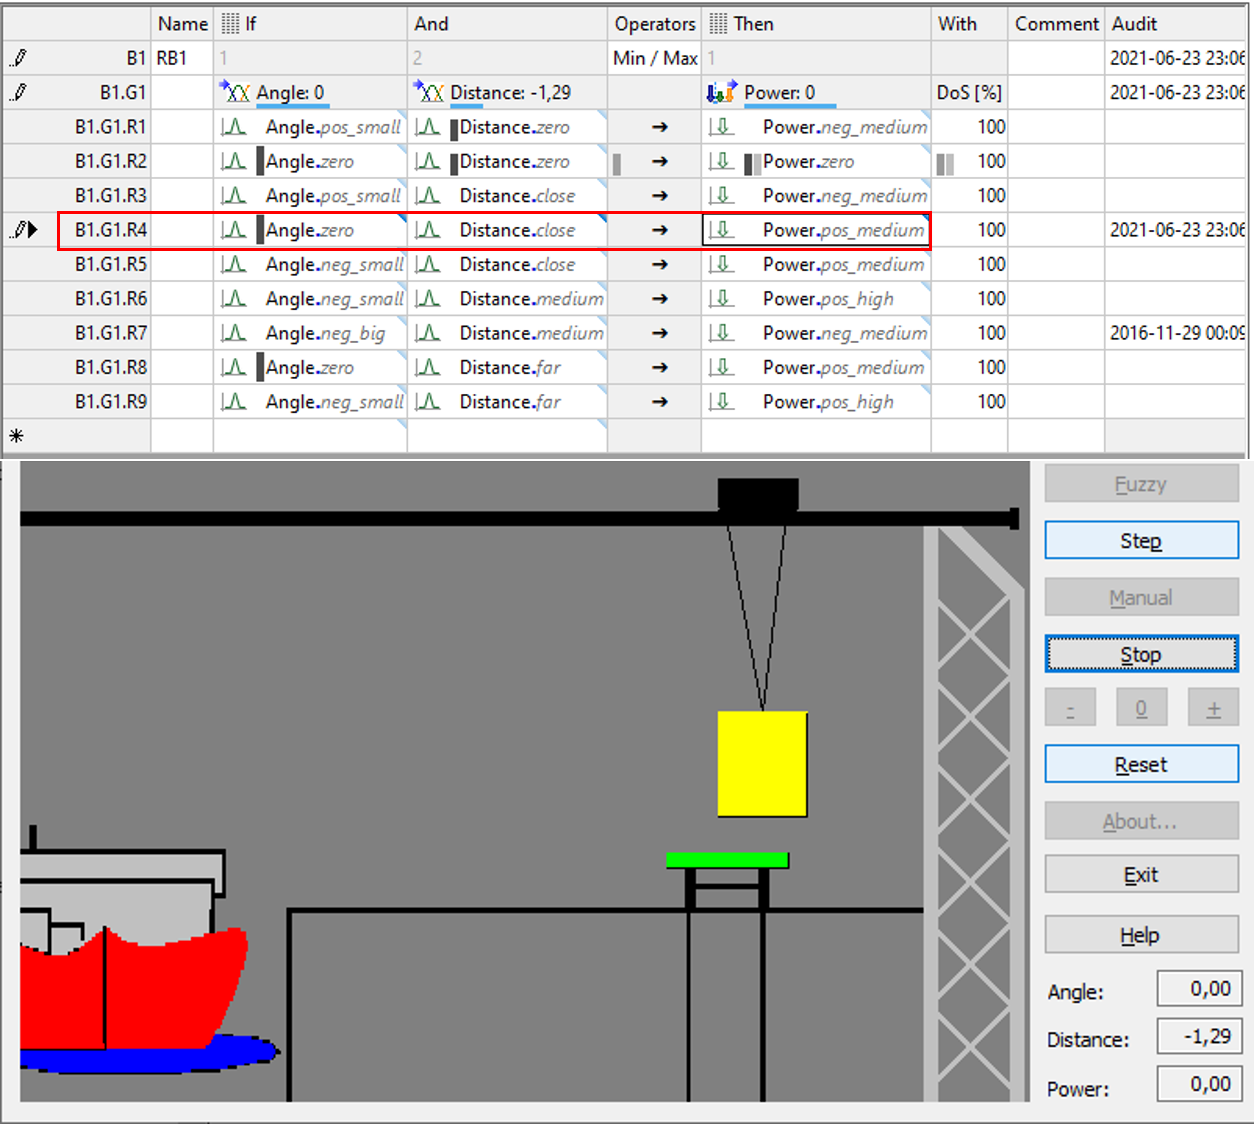
\includegraphics[width=0.7\linewidth]{Imagens/QR1/alteracao1}
	\caption{Resultado da primeira alteração}
	\label{fig:alteracao1}
\end{figure}

Com isso, o guindaste passou um pouco do local final adequado. Podemos tentar contrabalancear isso alterando a regra $(3)$ abaixo para $(4)$. 

\begin{align}
	Angle.pos\_small\&Distance.close&\to Power.neg\_medium\\
	Angle.pos\_small\&Distance.close&\to Power.neg\_high
\end{align}

O resultado encontra-se abaixo.
\begin{figure}[H]
	\centering
	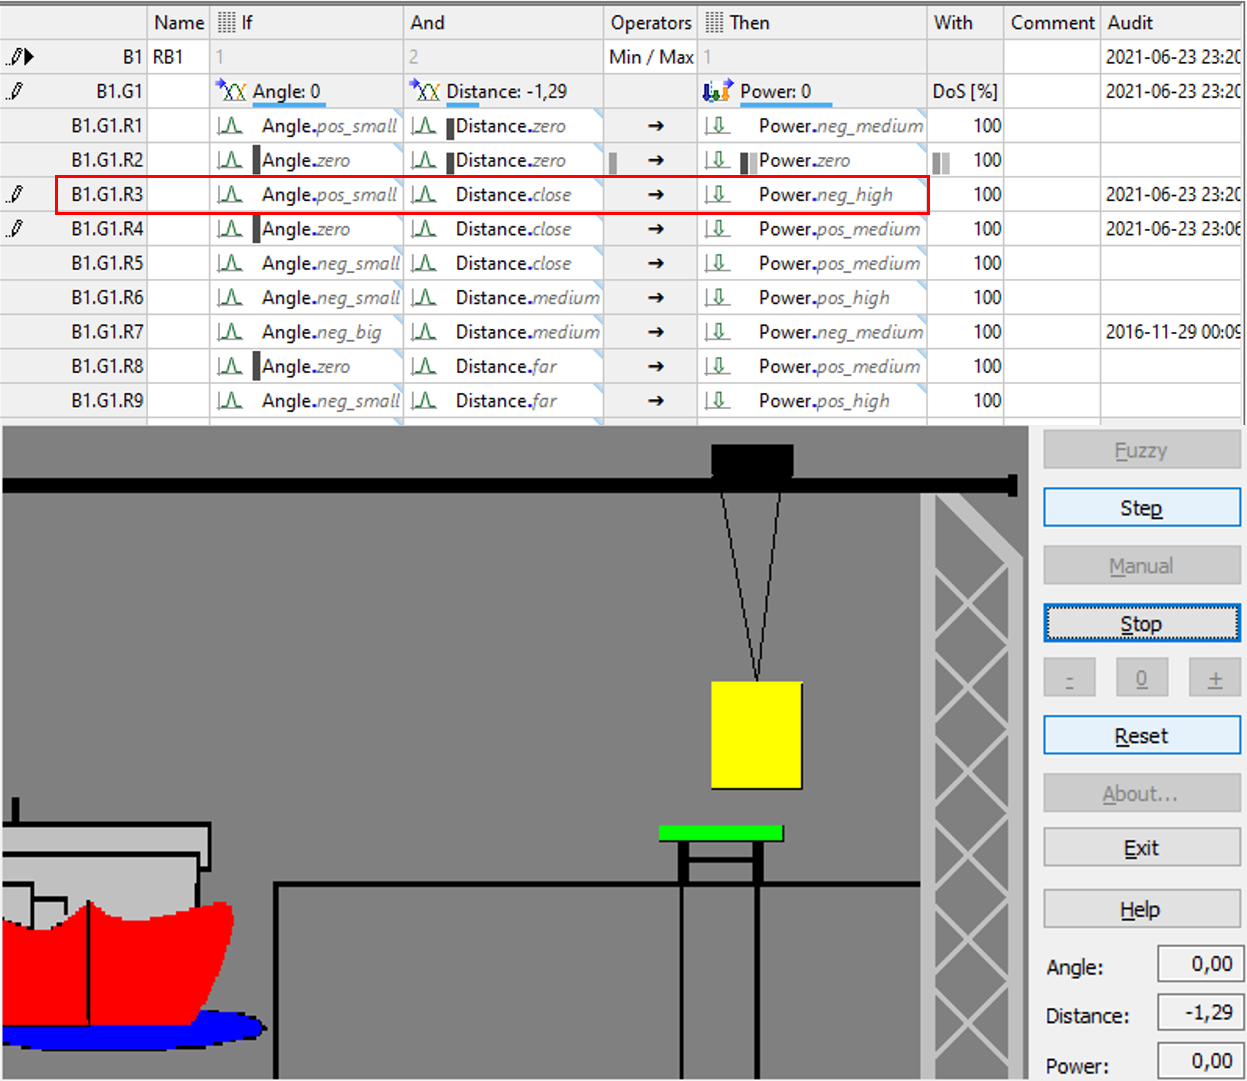
\includegraphics[width=0.7\linewidth]{Imagens/QR1/alteracao2}
	\caption{Resultado da segunda alteração}
	\label{fig:alteracao2}
\end{figure}

Pouca diferença é notada após essa segunda alteração. Sendo assim, ainda é necessária uma alteração que ou impeça o guindaste de passar da posição correta ou que, uma vez ultrapassada, faça o guindaste retornar. Como não existe na variável \textit{Distance} um valor que expresse a ultrapassagem. O enunciado estabelece que é proibida a exclusão de regras, mas não diz nada sobre a inclusão de novas regras. Sendo assim, foi incluída a regra $(5)$ abaixo para fazer com que o guindaste, se passar do local correto, volte um pouco.
\begin{equation}
	Angle.zero\&Distance.neg\_close\to Power.neg\_medium
\end{equation}

A figura abaixo exibe o resultado obtido com a inclusão dessa regra.

\begin{figure}[H]
	\centering
	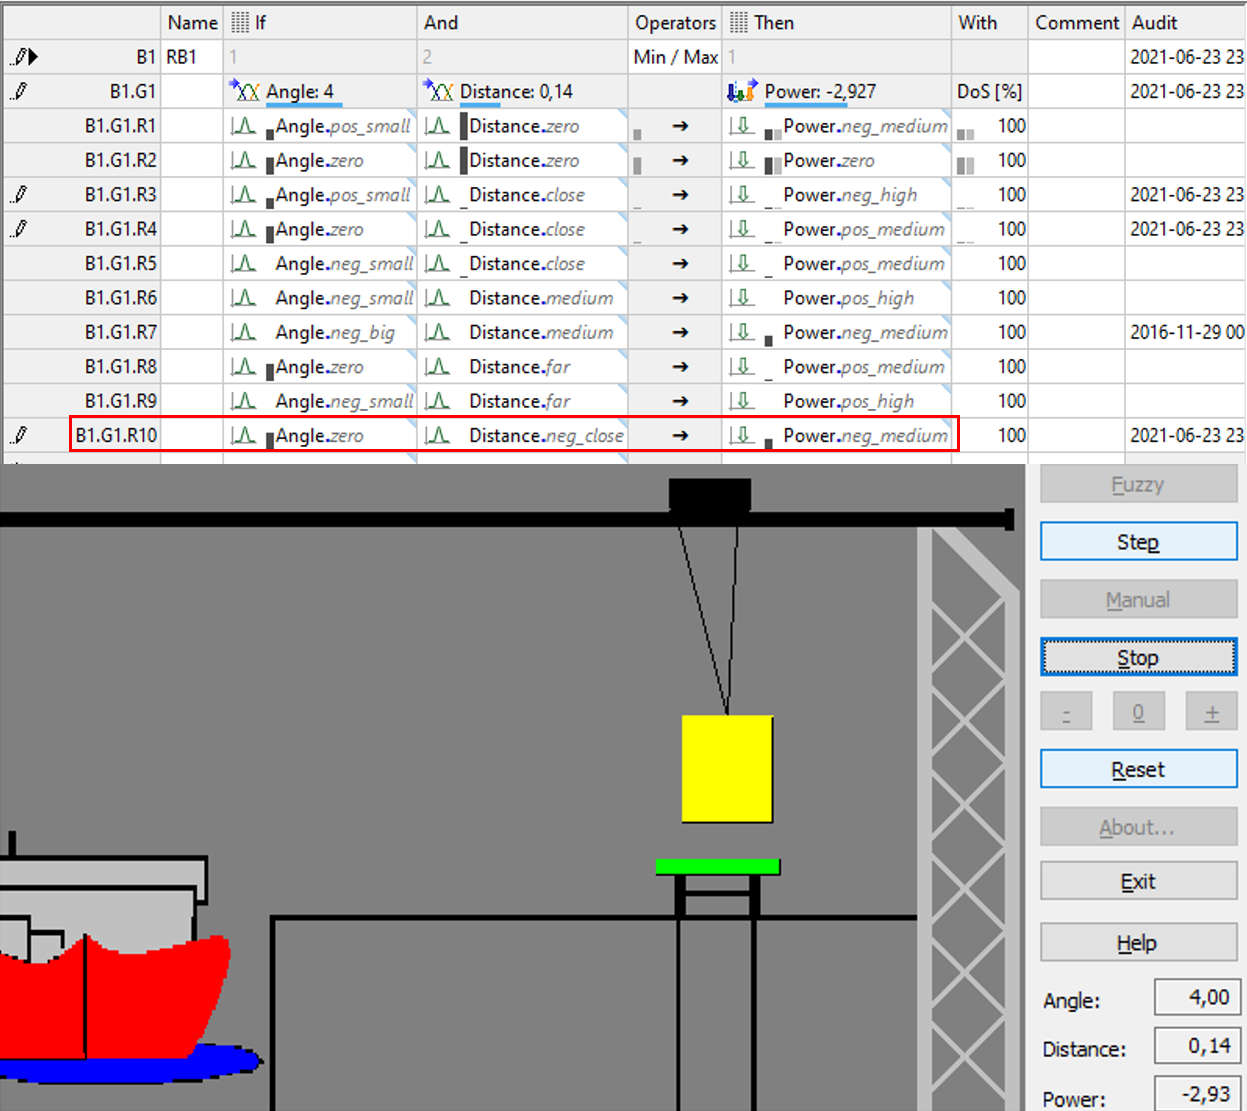
\includegraphics[width=0.7\linewidth]{Imagens/QR1/novaRegra1}
	\caption{Adição de nova regra}
	\label{fig:novaregra1}
\end{figure}

Nota-se que, com a adição dessa nova regra, a posição final do guindaste está muito próxima do ideal, com distância de $0.14$, sendo o ideal $0$.


\subsection{QR 2 - Exibindo estado inicial}

Assim como na seção anterior, a figura abaixo exibe as regras originais e a posição final original do guindaste.
\begin{figure}[H]
	\centering
	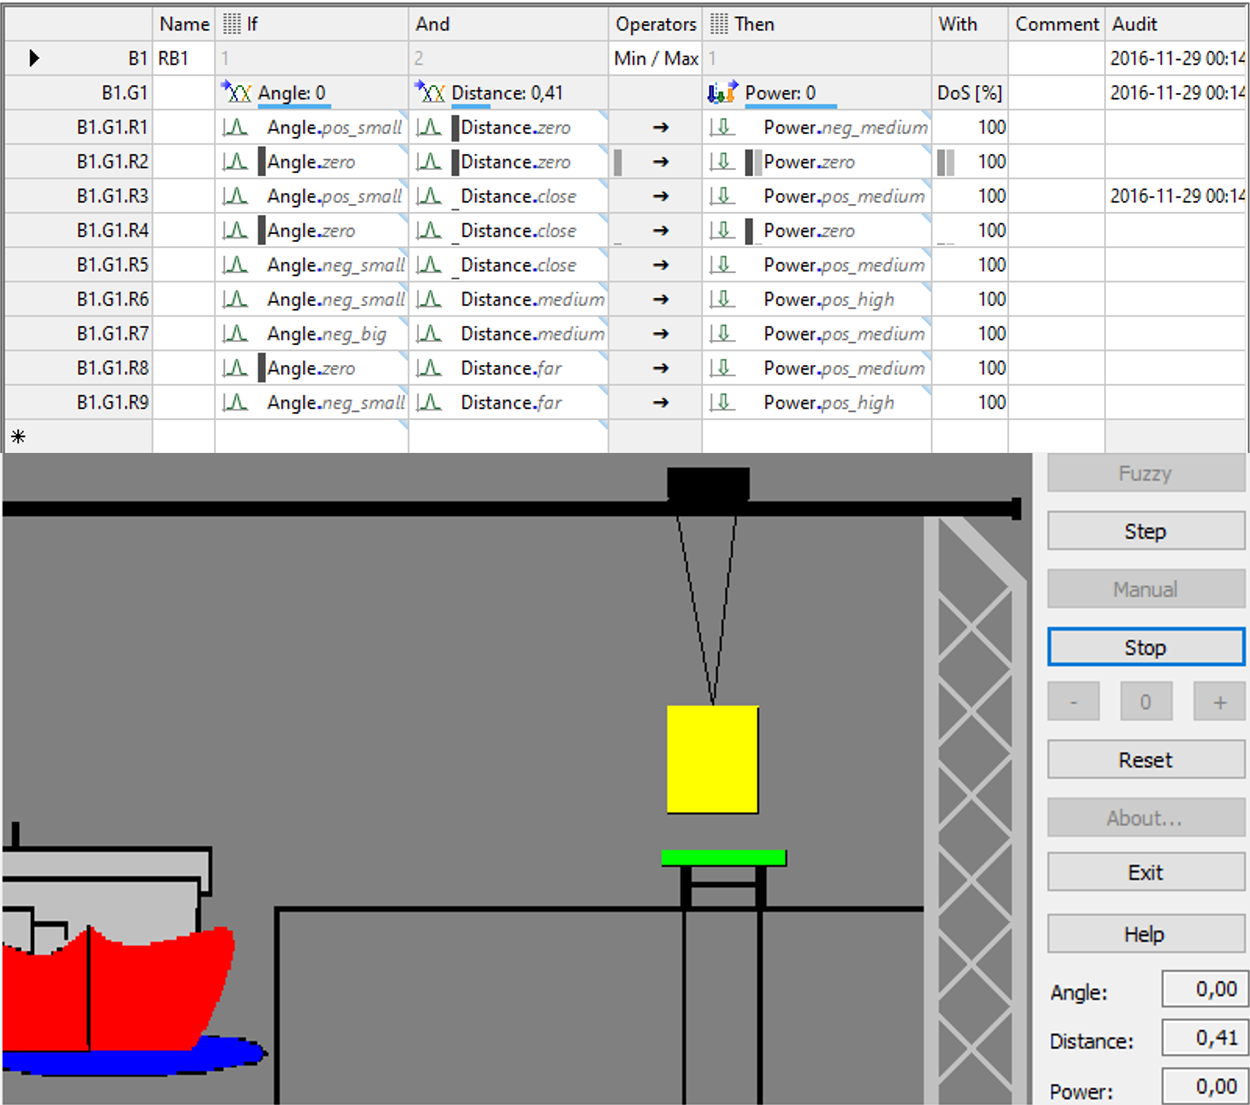
\includegraphics[width=0.7\linewidth]{Imagens/QR2/estadoOriginal}
	\caption{Regras originais e posição final original do guindaste}
	\label{fig:estadooriginal}
\end{figure}

Como pode ser percebido pelo canto inferior direito da figura \ref{fig:estadooriginal}, a posição final do guindaste está muito próxima da ideal. Dito isso, os ajustes que devem ser feitos nas regras devem estar mais relacionados com ajustes finos e finais, isto é, ajustes das regras que envolvem a variável \textit{Angle} em seus valores \textit{zero}, \textit{neg\_small} e \textit{pos\_small} e a variável \textit{Distance} em seus valores \textit{zero}, \textit{close} e \textit{neg\_close}. Além disso, a alteração nas regras deve fazer o guindaste andar um pouco mais para a direita.

\subsection{QR 2 - Alteração de Regras}

A primeira alteração a ser feita é trocar a regra $(6)$ pela regra $(7)$ abaixo.

\begin{align}
	Angle.neg\_small\&Distance.close&\to Power.pos\_medium\\
	Angle.neg\_small\&Distance.close&\to Power.neg\_medium
\end{align}

O que se espera com essa alteração é, quando o guindaste estiver muito próximo ao local desejado e com ângulo pequeno negativo, isto é, um pouco à direita do local desejado, ao invés de colocar potência positiva, que empurraria o guindaste mais para a direita, colocar potência negativa para trazê-lo um pouco mais para a esquerda. O resultado dessa alteração está exibido na figura abaixo.
\begin{figure}[H]
	\centering
	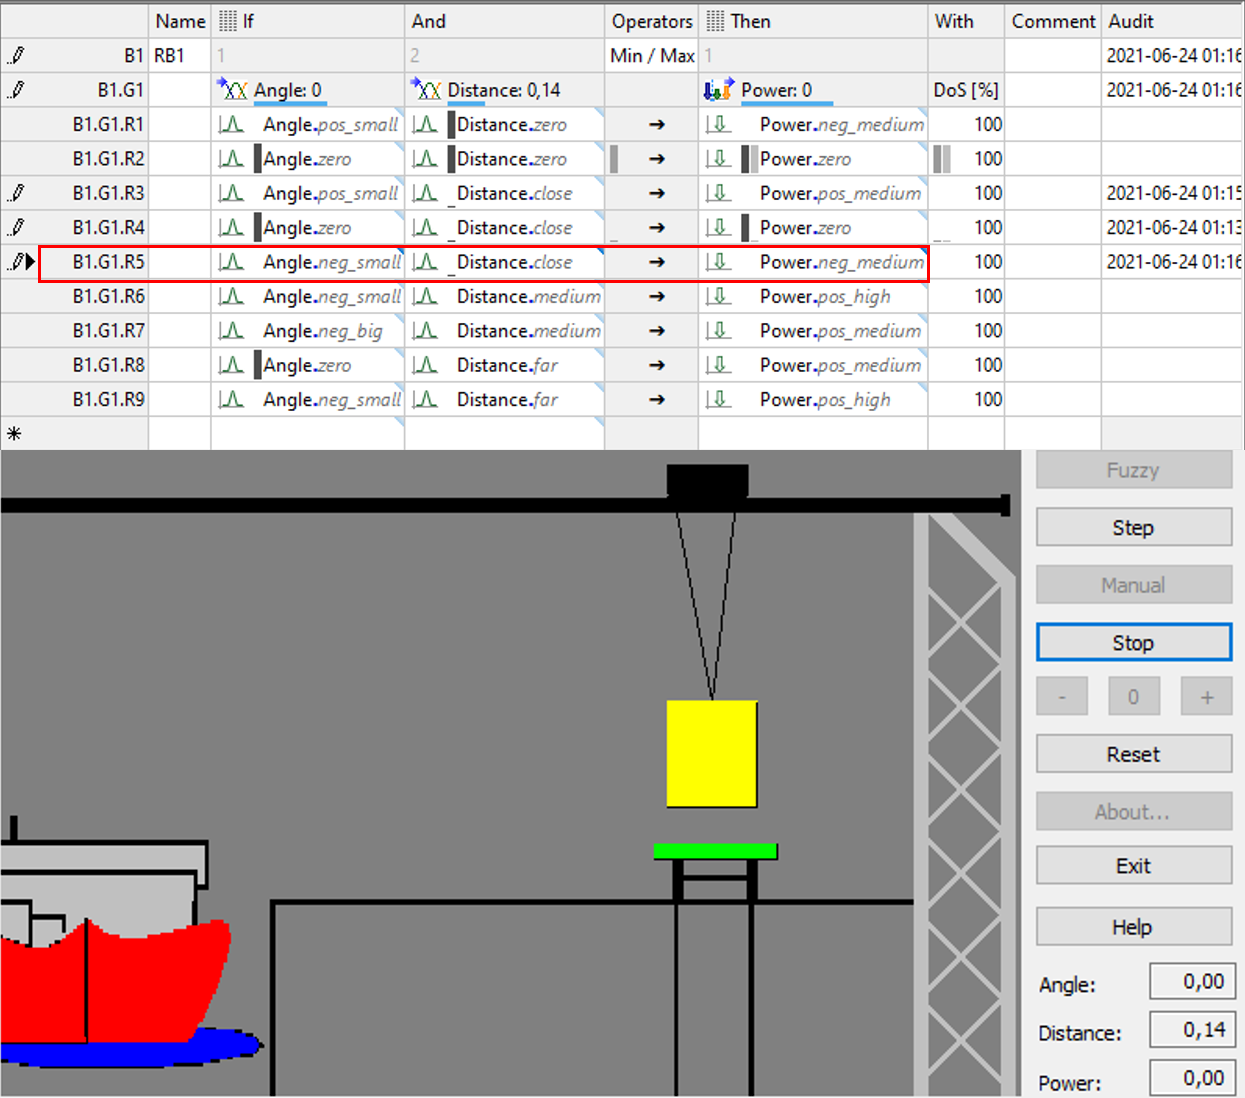
\includegraphics[width=0.8\linewidth]{Imagens/QR2/alteracao1}
	\caption{Alteração 1}
	\label{fig:alteracao1qr2}
\end{figure}

Como pode ser visto, a distância final está mais próxima da desejada, uma vez que o valor exibido caiu de $0.41$ para $0.14$, enquanto que o ângulo permaneceu em zero.

\section{Parte 2 - Problema Financiamento Imobiliário}

\subsection{Comentários Iniciais}

Primeiramente, o valor das variáveis para a minha matrícula, 1810764, são:
\begin{itemize}
	\item vl\_Localização = 50
	\item vl\_nivel\_Receita = 50
	\item vl\_Padrao\_Obra = 71
	\item vl\_Patrimonio = 58
	\item vl\_taxa\_Juros = 50	
\end{itemize}

O sistema de inferência fuzzy a ser criado segue o que está descrito no material disponibilizado na plataforma EAD e o que foi mostrado em aula. Sendo assim, podemos definir esse sistema de inferência assim como mostra a figura abaixo.
\begin{figure}[H]
	\centering
	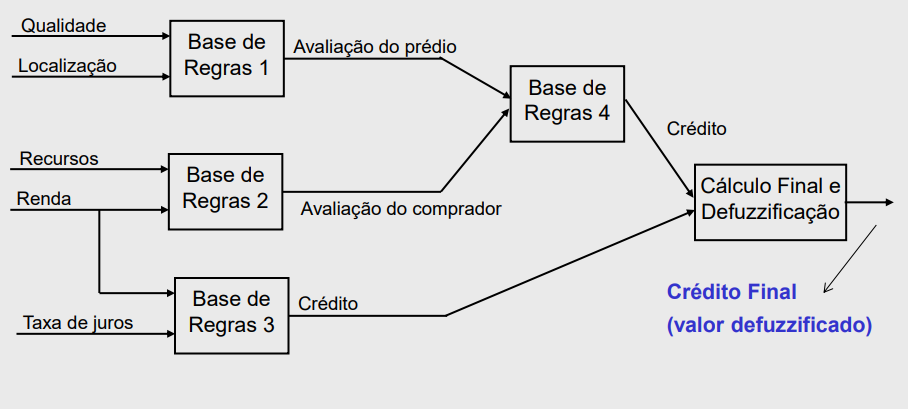
\includegraphics[width=0.9\linewidth]{Imagens/financiamento/esquemaSIF}
	\caption{Esquema do sistema de inferêcia fuzzy implementado}
	\label{fig:esquemasif}
\end{figure}

As variáveis de entrada \textit{vl\_Localização} e \textit{vl\_Padrao\_Obra} são usadas para definir a variável intermediária \textit{aval\_predio}, cuja base de dados pode ser a base 1 da figura \ref{fig:esquemasif}. As variáveis \textit{vl\_nivel\_Receita} e \textit{vl\_Patrimonio}, por sua vez, são usadas para definir a variável intermediária \textit{aval\_comprador} por meio de base de regras 2. Por fim, as variáveis \textit{vl\_taxa\_Juros} e \textit{vl\_Patrimonio} são usadas, via base de regras 3, para definir já a variável de saída \textit{credito\_fornecido}. As variáveis intermediárias \textit{aval\_predio} e \textit{aval\_comprador} são usadas, via base de regras 4, para definir a variável de saída, \textit{credito\_fornecido}.

\subsection{Montando o Sistema de Inferência Fuzzy}

Comecemos montando o sistema de inferência assim como descrito na figura \ref{fig:esquemasif}. Para isso, ainda é usado o \textit{FuzzyTech} e o arquivo disponibilizado na plataforma EAD. O \textit{SIF} montado é apresentado abaixo.
\begin{figure}[H]
	\centering
	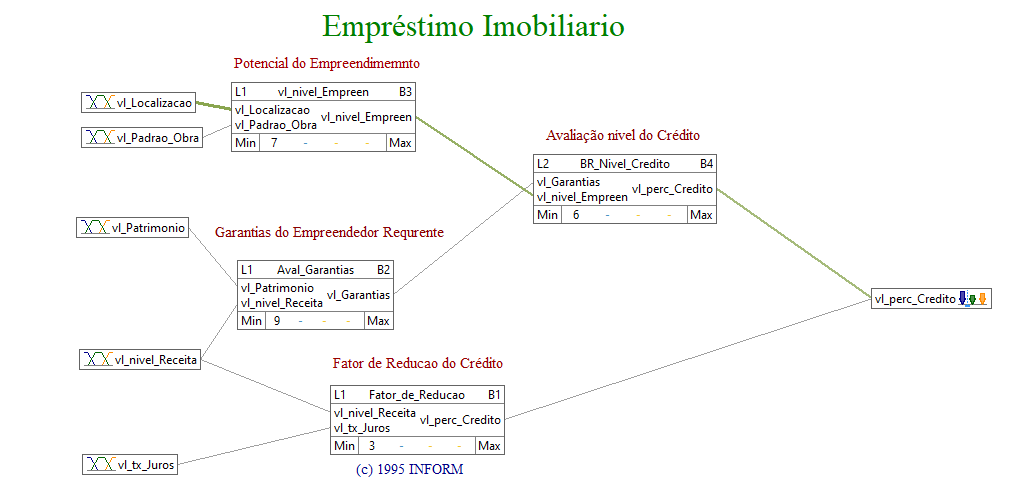
\includegraphics[width=0.9\linewidth]{Imagens/financiamento/SIF_FuzzyTech}
	\caption{SIF do Problema, disponibilizado no EAD}
	\label{fig:siffuzzytech}
\end{figure}

A figura abaixo exibe os valores linguísticos das variáveis de entrada e, logo abaixo, as regras originais.
\begin{figure}[H]
	\centering
	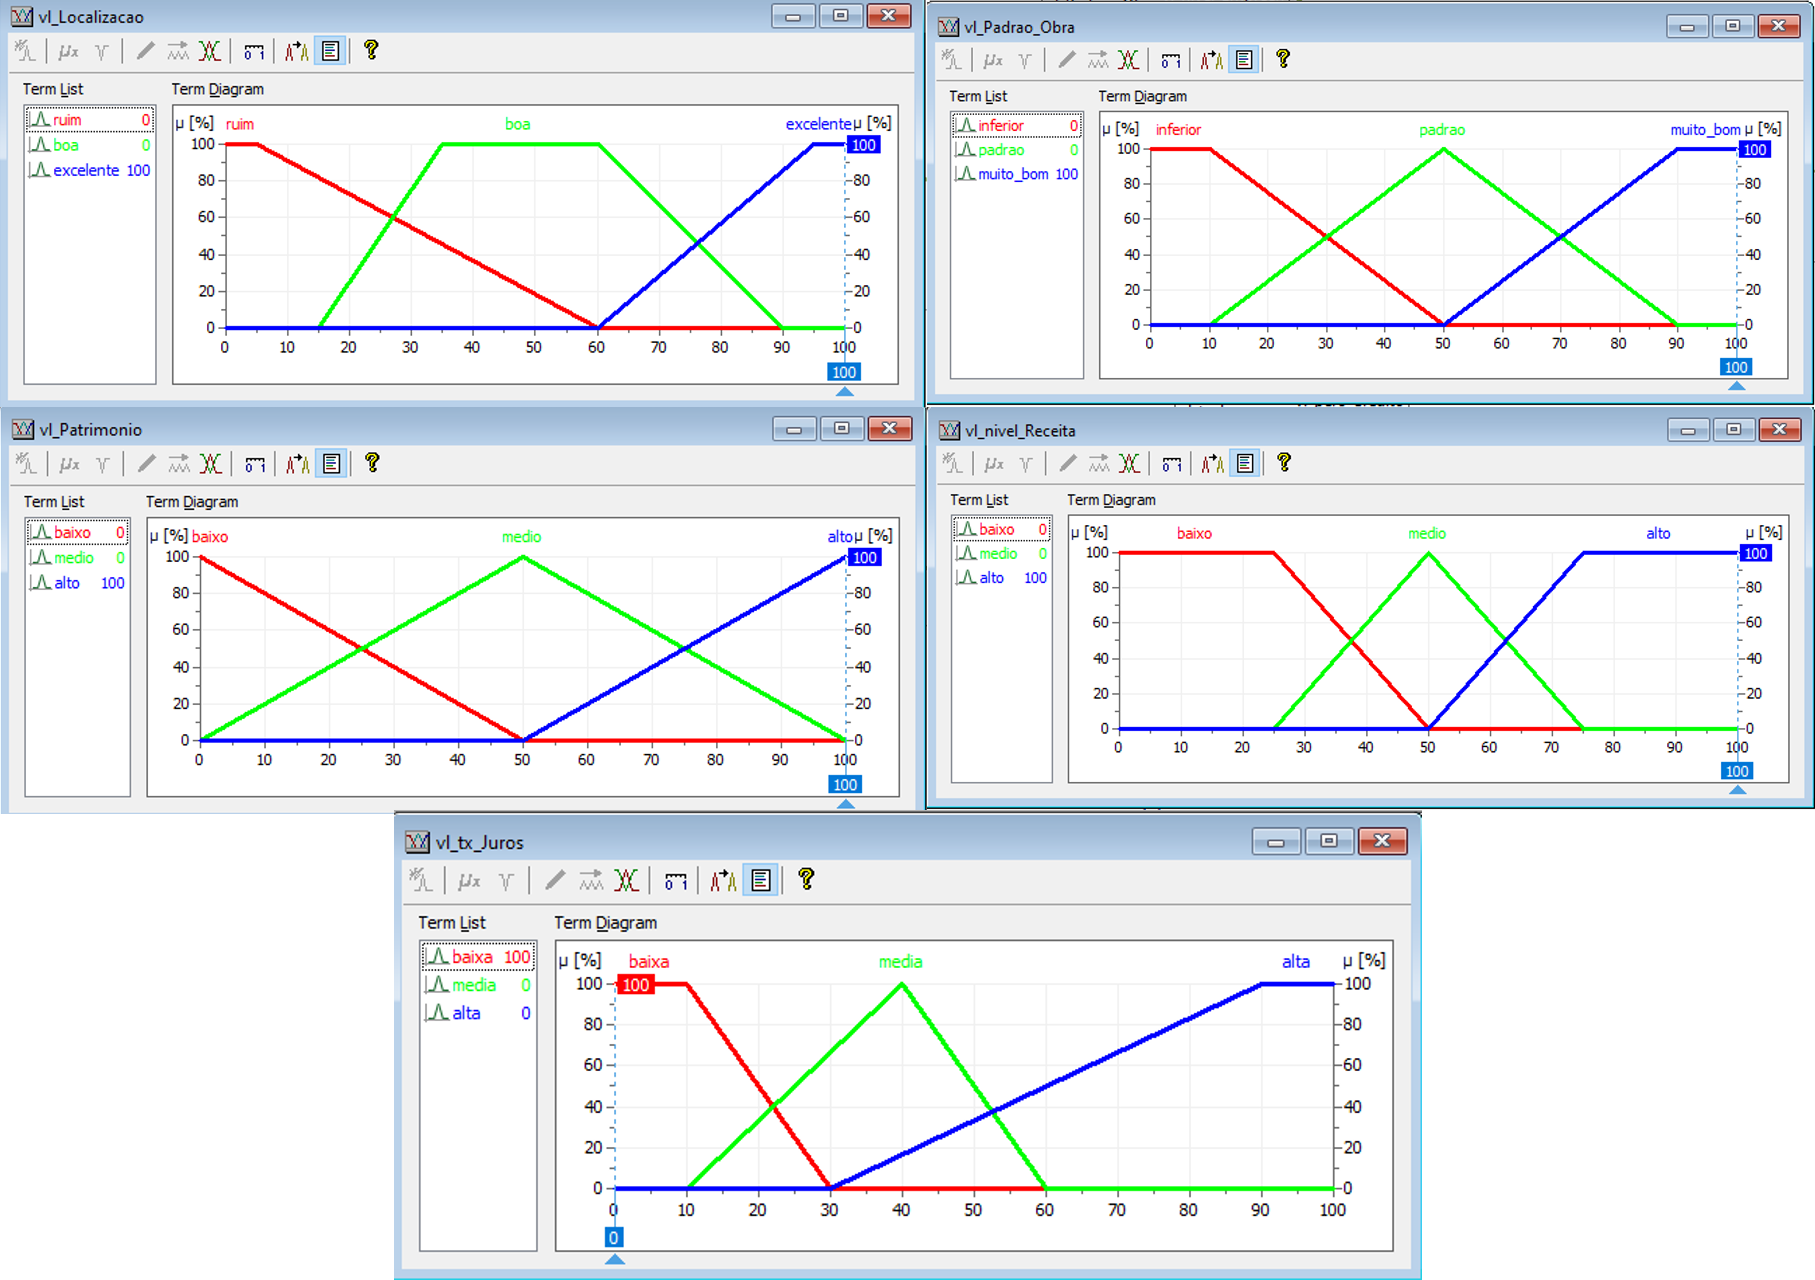
\includegraphics[width=0.9\linewidth]{Imagens/financiamento/VariaveisOriginais}
	\caption{Regras originais do SIF}
	\label{fig:variaveisoriginais}
\end{figure}

\begin{figure}[H]
	\centering
	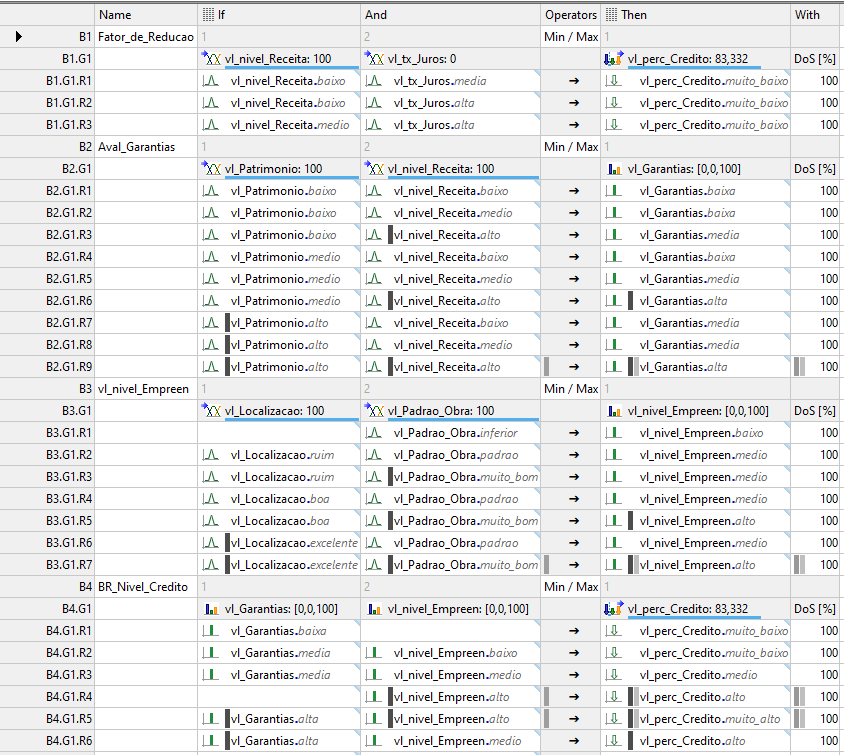
\includegraphics[width=0.8\linewidth]{Imagens/financiamento/RegrasOriginais}
	\caption{Regras Originais dos 4 blocos de regras}
	\label{fig:regrasoriginaisFinanciamento}
\end{figure}

Por fim, a figura abaixo exibe os conjuntos fuzzy, implementados como \textit{singletons} da variável de saída.
\begin{figure}[H]
	\centering
	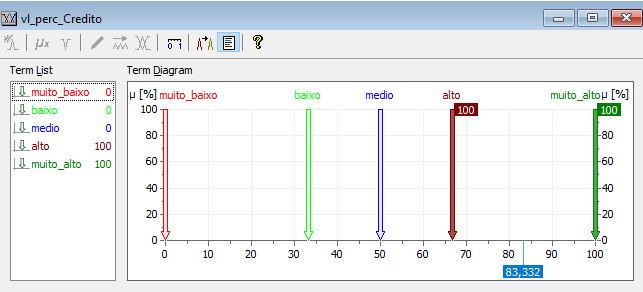
\includegraphics[width=0.7\linewidth]{Imagens/financiamento/CreditoFinalOriginal}
	\caption{Conjuntos fuzzy de saída}
	\label{fig:creditofinaloriginal}
\end{figure}

Como o enunciado do trabalho solicita apenas os cálculos das saídas e a resposta final do sistema, \textbf{não foram alteradas} as regras e conjuntos fuzzy do arquivo disponibilizado na plataforma EAD. Foram apenas realizados os cálculos com base nos parâmetros originais do arquivo.

\subsection{Respostas Manuais}

Será utilizado o operador \textbf{mínimo} para a norma-t do \textit{modus ponens generalizado}, para a implicação e para o conectivo \textit{e}. Para o conectivo \textbf{ou} será usado o operador \textbf{max}.

Vamos fazer a inferência por bloco de regras. Primeiramente, dados os valores das variáveis de minha matricula, cada variável possui grau de pertinência diferente de zero para os seguintes conjuntos:

\begin{itemize}
	\item vl\_Localização = 50 $\to$ \textit{boa(100\%)} e \textit{ruim(18\%)}
	\item vl\_Padrao\_Obra = 71 $\to$ \textit{padrão(48\%)} e \textit{muito\_bom(52\%)}
	\item vl\_Patrimonio = 58 $\to$ \textit{médio(84\%)} e \textit{alto(16\%)}
	\item vl\_nivel\_Receita = 50 $\to$ \textit{médio(100\%)}
	\item vl\_taxa\_Juros = 50	$\to$ \textit{média(50\%)} e \textit{alta(33\%)}
\end{itemize}

Comecemos pelo bloco de regras \textit{Aval\_Garantias}. Com base nos valores de função de pertinência acima, as regras ativadas desse bloco são:
\begin{align*}
	vl\_Patrimonio.baixo\&vl\_nivel\_Receita.medio&\to vl\_Garantias.baixa\\
	vl\_Patrimonio.medio\&vl\_nivel\_Receita.baixo&\to vl\_Garantias.baixa\\
	vl\_Patrimonio.medio\&vl\_nivel\_Receita.medio&\to vl\_Garantias.media\\
	vl\_Patrimonio.medio\&vl\_nivel\_Receita.alto&\to vl\_Garantias.alta\\
	vl\_Patrimonio.alto\&vl\_nivel\_Receita.baixo&\to vl\_Garantias.media\\
	vl\_Patrimonio.alto\&vl\_nivel\_Receita.medio&\to vl\_Garantias.media\\
	vl\_Patrimonio.alto\&vl\_nivel\_Receita.alto&\to vl\_Garantias.alta
\end{align*}

Sabendo o grau de pertinência de cada variável a cada conjunto, podemos escrever as operações abaixo:

\begin{align*}
	min(0,1)=0,&\mu_{baixa}(grnt)\\
	min(0.84,0)=0,&\mu_{baixa}(grnt)\\
	min(0.84,1)=0.84,&\mu_{media}(grnt)\\
	min(0.84,0)=0,&\mu_{alta}(grnt)\\
	min(0.16,0)=0,&\mu_{media}(grnt))\\
	min(0.16,1)=0.16,&\mu_{media}(grnt)\\
	min(0.16,0)=0,&\mu_{alta}(grnt)
\end{align*}


Fazendo a união das regras ou seja, o máximo de entre as regras acima, temos:
\begin{align*}
	\mu_{media}(grnt)=0.84\\
	\mu_{alta}(grnt)=0\\
	\mu_{baixa}(grnt)=0
\end{align*}

Façamos o mesmo procedimento para o bloco de regras \textit{vl\_nivel\_Empreend}:
\begin{align*}
	vl\_Localizacao.ruim\&vl\_nivel\_Padrao\_Obra.padrao&\to vl\_nivel\_Empreend.medio\\
	vl\_Localizacao.ruim\&vl\_nivel\_Padrao\_Obra.muito\_Bom&\to vl\_nivel\_Empreend.medio\\
	vl\_Localizacao.boa\&vl\_nivel\_Padrao\_Obra.padrao&\to vl\_nivel\_Empreend.medio\\
	vl\_Localizacao.boa\&vl\_nivel\_Padrao\_Obra.muito\_Bom&\to vl\_nivel\_Empreend.alto\\
	vl\_Localizacao.excelente\&vl\_nivel\_Padrao\_Obra.padrao&\to vl\_nivel\_Empreend.medio\\
	vl\_Localizacao.excelenteuim\&vl\_nivel\_Padrao\_Obra.muito\_Bom&\to vl\_nivel\_Empreend.alto
\end{align*}

\begin{align*}
	min(0.18,0.48)=0.18,&\mu_{medio}(nivel\_Empreend)\\
	min(0.18,0.52)=0.18,&\mu_{medio}(nivel\_Empreend)\\
	min(1,0.48)=0.48,&\mu_{medio}(nivel\_Empreend)\\
	min(1,0.52)=0.52,&\mu_{alto}(nivel\_Empreend)\\
	min(0,0.48)=0,&\mu_{medio}(nivel\_Empreend)\\
	min(0,0.52)=0,&\mu_{alto}(nivel\_Empreend)
\end{align*}

Fazendo a união, ou seja, o máximo de entre as regras acima, temos:
\begin{align*}
	\mu_{alto}(nivel\_Empreend)=0.52\\
	\mu_{medio}(nivel\_Empreend)=0.48
\end{align*}

Fazendo o mesmo procedimento para o bloco de regras \textit{Fator\_de\_Reducao}, temos:
\begin{align*}
	vl\_nivel\_Receita.baixo\&vl\_tx\_Juros.media&\to vl\_perc\_Credito.muito\_baixo\\
	vl\_nivel\_Receita.baixo\&vl\_tx\_Juros.alta&\to vl\_perc\_Credito.muito\_baixo\\
	vl\_nivel\_Receita.medio\&vl\_tx\_Juros.alta&\to vl\_perc\_Credito.muito\_baixo\\
\end{align*}
\begin{align*}
	min(0,0.5)=0,&\mu_{muito\_baixo}(perc\_Cred)\\
	min(0,0.33)=0,&\mu_{muito\_baixo}(perc\_Cre))\\
	min(1,0.33)=0.33,&\mu_{muito\_baixo}(perc\_Cred)
\end{align*}

Fazendo a união, ou seja, o máximo de entre as regras acima, temos:
\begin{equation*}
	\mu_{muito\_baixo}(perc\_Cred)=0.33
\end{equation*}

Por fim, o último bloco de regras, \textit{BR\_Nivel\_Credito}:
\begin{align*}
	vl\_Garantias.media\&vl\_nivel\_Empreen.baixo&\to vl\_perc\_Credito.muito\_baixo\\
	vl\_Garantias.media\&vl\_nivel\_Empreen.medio&\to vl\_perc\_Credito.medio\\
	vl_nivel\_Empreen.alto&\to vl\_perc\_Credito.alto\\
	vl\_Garantias.alta\&vl\_nivel\_Empreen.alto&\to vl\_perc\_Credito.muito_alto\\
	vl\_Garantias.alta\&vl\_nivel\_Empreen.medio&\to vl\_perc\_Credito.alto
\end{align*}
\begin{align*}
	min(\mu_{media}(grnt),\mu_{baixo}(nivel\_Empreend)),&\mu_{muito\_baixo}(perc\_Cred)\\
	min(\mu_{media}(grnt),\mu_{medio}(nivel\_Empreend)),&\mu_{medio}(perc\_Cred)\\
	min(\mu_{alto}(nivel\_Empreend),&\mu_{alto}(perc\_Cred))\\
	min(\mu_{alta}(grnt),\mu_{alto}(nivel\_Empreend)),&\mu_{muito\_alto}(perc\_Cred)\\
	min(\mu_{alta}(grnt),\mu_{medio}(nivel\_Empreend)),&\mu_{alto}(perc\_Cred)
\end{align*}

Substituindo valores:

\begin{align*}
	min(0.84,0)=0,&\mu_{muito\_baixo}(perc\_Cred)\\
	min(0.84,0.48)=0.48,&\mu_{medio}(perc\_Cred)\\
	min(0.52)=0.52,&\mu_{alto}(perc\_Cred)\\
	min(0,0.52)=0,&\mu_{muito\_alto}(perc\_Cred)\\
	min(0,0.48)=0,&\mu_{alto}(perc\_Cred)
\end{align*}

Fazendo a união, ou seja, o máximo de entre as regras acima, considerando o valor obtido $\mu_{muito\_baixo}(perc\_Cred)=0.33$ no bloco de regras \textit{Fator\_de\_Reducao}, temos, por fim:

\begin{align*}
	\mu_{muito\_baixo}(perc\_Cred)=0.33\\
	\mu_{medio}(perc\_Cred)=0.48\\
	\mu_{alto}(perc\_Cred)=0.52
\end{align*}

Uma vez obtidos os graus de pertinência da variável de saída, precisamos realizar a desfuzzificação. Para tal, calcularemos o centro de massa dessas variáveis. Note que esses valores de grau de pertinência são, exatamente, os calculados pelo \textit{FuzzyTech}, exibidos na figura \ref{fig:creditofinaloriginal}

\begin{equation*}
	Centroide=\dfrac{0.33\cdot0+0.48\cdot50+0.52\cdot66}{0.33+0.48+0.52}=43.85
\end{equation*}

Logo, o cliente em questão deve receber $43.85\%$ do limite máximo de crédito.
	
\subsection{Respostas FuzzyTech}

Utilizando as variáveis e regras definidas nas seções anteriores, usamos o \textit{FuzzyTech} para calcular a saída para fins de comparação com as contas manuais.

\begin{figure}[H]
	\centering
	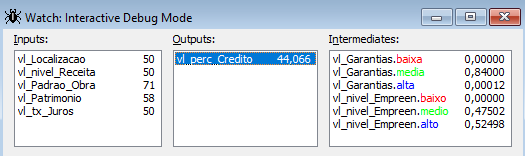
\includegraphics[width=0.8\linewidth]{Imagens/financiamento/ResultadoFinalOriginal}
	\caption{Quantidade de crédito recebida}
	\label{fig:resultadofinaloriginal}
\end{figure}

Note que o resultado está muito próximo do calculado. Um possível fonte de erro pode ser a análise dos gráficos para descobrir os valores dos graus de pertinência.

\end{document}